\lecture{12}{wed 12 oct 11:00}{Demand Elasticity}
\section{Price Elasticity of Demand}
\begin{definition}
    \textbf{Elasticity} is the responsiveness to change. In laymans terms, you can safely see the elasticity is the slope of the line.
\end{definition}
\begin{itemize}
    \item Price Elasticity of Demand
        \begin{itemize}
            \item Consumers' responsiveness to a change in price
        \end{itemize}
    \item Income Elasticity
        \begin{itemize}
            \item Consumers' responsiveness to a change in income
        \end{itemize}
    \item Cross Price Elasticity
        \begin{itemize}
            \item Consumers' responsiveness to a change in the price of a related good
        \end{itemize}
    \item Price Elasticity of Supply
        \begin{itemize}
            \item Suppliers' responsiveness to a change in price
        \end{itemize}
\end{itemize}

So for now we will focus on elasticity with demand. So we know that the law of demand tells us the price and quantity demanded are inverselt related, which leads to the downword slope. What we dont know is how much the quantity demanded changes as result in a price drop. \textbf{That is what} elasticity is. 

\begin{figure}[h!]
\begin{center}
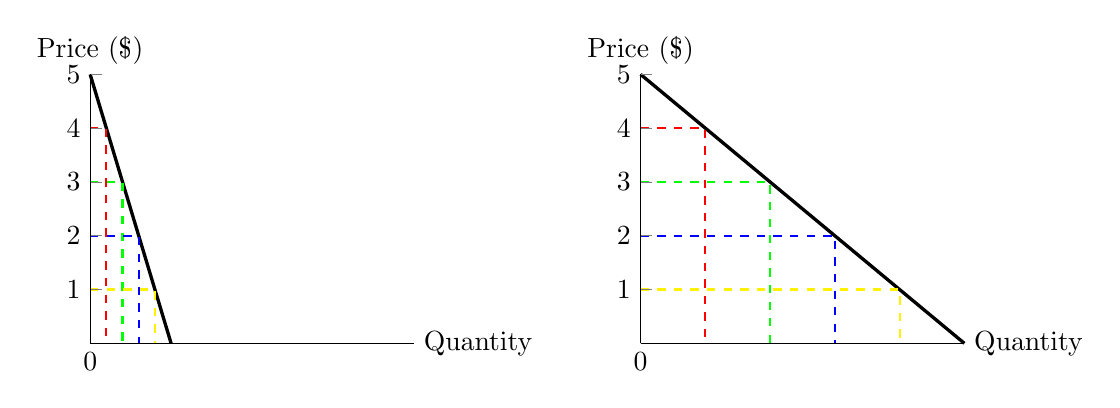
\begin{tikzpicture}
\begin{axis}[
scale=0.6,
xmin = 0, xmax = 10,
ymin = 0, ymax = 5, 
axis lines* = left,
xtick = {0}, ytick = {1,2,3,4,5},
axis on top, 
clip = false,
]

\addplot[color = black, very thick] coordinates {(0,5) (2.5,0)};

\addplot[color = red, dashed, thick] coordinates {(0,4) (0.5,4) (0.5,0)};
\addplot[color = green, dashed, thick] coordinates {(0,3) (1,3) (1,0)};
\addplot[color = blue, dashed, thick] coordinates {(0,2) (1.5, 2) (1.5, 0)};
\addplot[color = yellow, dashed, thick] coordinates {(0,1) (2,1) (2,0)};

\node [above] at (current axis.above origin) {Price (\$)};
\node [right] at (current axis.right of origin) {Quantity};

\end{axis}
\begin{axis}[
scale=0.6,
xmin = 0, xmax = 10,
ymin = 0, ymax = 5,
axis lines* = left,
xtick = {0}, ytick = {1,2,3,4,5},
axis on top,
clip = false,
shift = {(axis cs: 17, 0)},
]

\addplot[color = black, very thick] coordinates {(0,5) (10,0)};

\addplot[color = red, dashed, thick] coordinates {(0,4) (2,4) (2,0)};
\addplot[color = green, dashed, thick] coordinates {(0,3) (4,3) (4,0)};
\addplot[color = blue, dashed, thick] coordinates {(0,2) (6,2) (6, 0)};
\addplot[color = yellow, dashed, thick] coordinates {(0,1) (8,1) (8,0)};

\node [above] at (current axis.above origin) {Price (\$)};
\node [right] at (current axis.right of origin) {Quantity};

\end{axis}
\end{tikzpicture}
\caption{Elasticity}
\label{fig:slope}
\end{center}
\end{figure}

The slope of the line will tell how much quantity demanded will change when the \textbf{price} changes. What can affect the slope? Well things like income, necessity vs luxury items, or substitutes and their availabilty can affect the slope. 

How to calculate elasticity, sadly it isnt as simple as finding the slope, instead you will either need to find the \% change formula or the Total Revenue Test. The income effect and substitution effect can determine the price elasticity of demand.
\begin{example}
    Lets look at some examples:
    \textbf{Substitution Effect}\\
    Lets see a bag of navel oranges, navel oranges are a specific type of oranges, and thus have lots of substitutes. So naval oranges is price elastic. Now what about gasoline, gasoline has no substitutes so its fairly price inelastic. \\
    \textbf{Income Effect}\\
    Lets look at compact SUV's, which makes up a large part of the middle class income, so its price elastic. People will wait till they get a good price on the vehicle. Candy bars on the other hand, are so inexpensive that they make up a small part of the middle class income, so its price inelastic. You would be willing to pay higher prices on the candy bar since it is such a small part of your income. 
\end{example}

In most cases, the income effect with reinforce the substitution effect. In normal goods they reinforce each other, but in the case of inferior goods, they contradict each other. When price goes up, quanity demanded will also go up in inferior goods. 

Now let me lay the ground work for your understanding of Elasticity of Demand.
\[
    E_D < 1 = \text{inelastic}\\
    E_D = 1 = \text{unit elastic}\\
    E_D > 1 = \text{elastic}
.\] 

Now lemme clarify how something inelastic, unit elastic, or elastic graph would look. Make sure to include arrows to indicate change, but since this is a pdf and its quite difficult to draw arrows, everything will move from subscript 1 to 2.

\textbf{Perfectly Inelastic Demand}\\

\begin{figure}[h!]
\begin{center}
\begin{tikzpicture}
\begin{axis}[
scale=0.6,
xmin = 0, xmax = 10,
ymin = 0, ymax = 10, 
axis lines* = left,
xtick = \empty, ytick = \empty,
axis on top, 
clip = false,
]

\addplot[color = black, very thick] coordinates {(3,0) (3,10)};
\addplot[color = black, dashed, thick] coordinates {(0,7) (3,7)};
\addplot[color = black, dashed, thick] coordinates {(0,4) (3,4)};

\node[left = 5pt] at (0,7) {$P_1$};
\node[left = 5pt] at (0,4) {$P_2$};
\node[below = 5pt] at (3,0) {$Q_1$};

\node [above] at (current axis.above origin) {$P$};  
\node [right] at (current axis.right of origin) {$Q$};
\node [above = 5pt] at (3,10) {$D$};

\end{axis}
\end{tikzpicture}
\end{center}
\end{figure}

Whats happening here is that no matter how much the price falls, the quantity does not change. This would make $E_D = 0$. This should help explain that inelastic is when the quantity does not change drastically. 

\textbf{Relatively Inelastic Demand}\\
I am pretty lazy to draw this in my software, but its a steep slope in mathematics. When price falls, the quantity rises less than the change in price. Remember this is being done in percents, so if price falls by 10\%, the quantity will rise less than 10\% in this scenario. 

\textbf{Unit Elastic} \\
\begin{figure}[h!]
\begin{center}
\begin{tikzpicture}
\begin{axis}[
scale=0.65,
xmin = 0, xmax = 10,
ymin = 0, ymax = 10,
axis lines* = left,
xtick = \empty, ytick = \empty,
axis on top,
clip = false,
]

\addplot[color = black, very thick] coordinates {(0, 10) (10, 0)};
\addplot[color = black, dashed, thick] coordinates {(0, 6) (4, 6) (4, 0)};
\addplot[color = black, dashed, thick] coordinates {(0, 4) (6, 4) (6, 0)};

\node[left = 5pt] at (0, 6) { P₁ };
\node[left = 5pt] at (0, 4) { P₂ };
\node[below = 5pt] at (4, 0) { Q₁ };
\node[below = 5pt] at (6, 0) {$Q_2$};

\node [above] at (current axis.above origin) {P};
\node [right] at (current axis.right of origin) {Q};
\node [above = 5pt, fill = white] at (0, 10) {D};

\end{axis}
\end{tikzpicture}
\label{fig:unitelastic}
\end{center}
\end{figure} 

  With this graph, unit elastic means that however much the price falls, the quantity will rise by. So if the price falls by 10\% then the quantity will rise by 10\%. This is usually a 45 degree angle on the graph, and its where the price effect = the quantity effect. $E_D = 1$

  \textbf{Perfectly Elastic Demand}\\
  \begin{figure}[h!]
  \begin{center}
  \begin{tikzpicture}
  \begin{axis}[
  scale=0.7,
  xmin = 0, xmax = 10,
  ymin = 0, ymax = 10,
  axis lines* = left,
  xtick = \empty, ytick = \empty,
  axis on top,
  clip = false,
  ]

  \addplot[color = black, very thick] coordinates {(0,5) (10,5)};
  \addplot[color = black, dashed, thick] coordinates {(4,0) (4,5)};
  \addplot[color = black, dashed, thick] coordinates {(7,0) (7,5)};

  \node[left = 5pt] at (0,5) {$P_2 = P_1$};
  \node[below = 5pt] at (4,0) { Q₁ };
  \node[below = 5pt] at (7,0) {$Q_2$};
  
  \node [above] at (current axis.above origin) {P};
  \node [right] at (current axis.right of origin) {Q};
  \node [above = 5pt] at (10,5) {D};

  \end{axis}
  \end{tikzpicture}
  \end{center}
  \end{figure} 

  This represents a perfectly elastic demand, where at the current price you can get as many people that you want to buy it. But if the price drops, then no-one will buy it. This results in a $E_D = \infty$ and is a horizontal slope. 

\textbf{Relatively Elastic Demand}\\
Since I am still lazy, I will just explain what it is. It is when $E_D > 1$, and its more of a flat slope. If price falls by 10\%, then the quantity will rise more than 10\%. The quantity will rise more than the price has fallen. 

As a summary of everything, inelastic means that the price changes more than the quantity will. If price falls more than quanity rises, its inelastic. If its unit elastic, price and quanity will equal. If price falls, quanity will rise the same amount. Elastic means that quantity will be greater than price. If price falls, the quantity risen will be greater than what price fell. Perfectly inelastic just means at no change in price, the quantity is infinite, meaning you can already get everyone at that price. I mentioned $E_D$ in this section, and you will learn how to calculate this in the next lecture. 

